\documentclass[a4paper, 10pt]{article}

\usepackage[utf8]{inputenc}
\usepackage[spanish]{babel}
\usepackage{graphicx}
\usepackage{geometry}
\usepackage{listings}
\usepackage{amsmath}
\usepackage{amsfonts}
\usepackage{amssymb}
\usepackage{caratula}
\usepackage[section]{placeins}
\usepackage{titlesec}
\usepackage[colorlinks=true,linkcolor=blue,urlcolor=black,bookmarksopen=true]{hyperref}
\usepackage{bookmark}

\newcommand{\Z}{\mathbb{Z}}
\def\code#1{\texttt{#1}}
\newcommand\tab[1][0.5cm]{\hspace*{#1}}

\geometry{a4paper, margin=0.7in}

\begin{document}
    %Caratula
    \pagenumbering{gobble}
    \newpage

    \begin{center}
        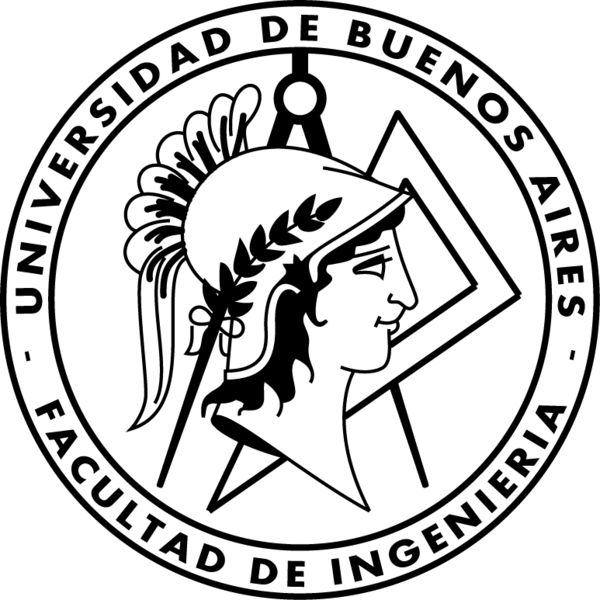
\includegraphics[width=7.5cm, height=7.5cm]{../images/logo}
    \end{center}

    \materia{Organización de Datos}
    \submateria{Segundo Cuatrimestre 2017}
    \titulo{Trabajo Práctico 1}

    \integrante{Rodrigo De Rosa}{97799}{rodrigoderosa@outlook.com}
    \integrante{Marcos Schapira}{97934}{schapiramarcos@gmail.com}
    \integrante{Facundo Guerrero}{97981}{facundoiguerrero@gmail.com}
    \maketitle
    %Fin caratula
    %Table of contents
    \newpage
    \pagenumbering{roman}
    \tableofcontents
    %Fin table of contents
    %Informe
    \newpage
	\pagenumbering{arabic}
	\part{Análisis del tipo de las propiedades}
		\section{Tipos de propiedades y sus superficies}
			\subsection{¿Dónde están las propiedades más chicas según su tipo?}	
				\subsubsection{Casas}
					Para las casas, el \emph{Bottom 5} está compuesto por los siguientes barrios:
					\begin{center}
						\begin{tabular}{ |c|c|c| }
							\hline
							\multicolumn{3}{|c|}{Superficie promedio de las casas por barrio}\\
							\hline
							\hline
							Puesto & Barrio & Superficie [$m^2$]\\
							\hline
							5 & José León Suarez & 176\\
							4 & Remedios de Escalada & 175\\
							3 & Lanús & 173\\
							2 & Munro & 161 \\
							1 & Llavallol & 160\\
							\hline
						\end{tabular}
					\end{center}
					\tab Aquí podemos ver que incluso el barrio con el promedio más pequeño tiene una superficie promedio mayor
					a la de los barrios con mayor superficie promedio en el caso de los PHs y los departamentos. \\
					\tab Si se grafican estos cinco barrios:
					\begin{center}
   		    				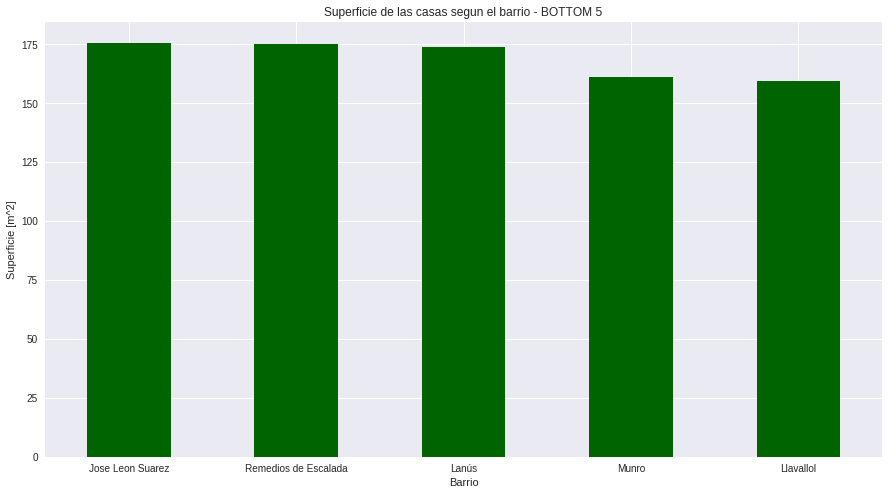
\includegraphics[width=\textwidth]{../images/houseSurfaceBottomBar}
				  	\end{center}
				  	\tab Se puede ver la poca diferencia que hay entre cada uno de los barrios, siendo entre los cinco de sólo
				  	$16m^2$ mientras que entre los primeros tres hay sólo $3m^2$ de diferencia. \\
				  	\tab En cuanto a la ubicación geográfica de estos barrios, podemos ver el siguiente mapa:
				  	\begin{center}
   		    				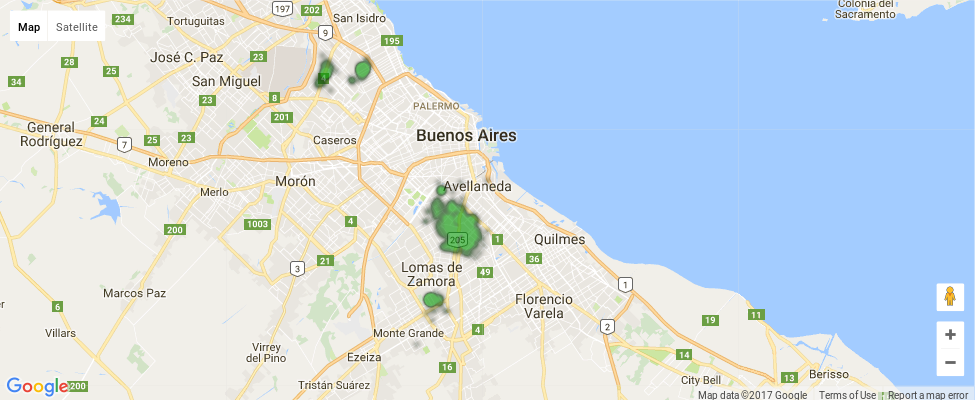
\includegraphics[width=\textwidth]{../images/houseSurfaceBottomMap}
				  	\end{center}
				  	\tab Aquí se observa que los barrios con menor promedio de superficie para las casas, al igual que ellos con
				  	mayor promedio, se encuentra en la provincia de Buenos Aires, divido entre el sur y el norte. Tanto para el
				  	sur como para el norte podemos ver que, salvo por Munro, no son barrios del primer cordón del conurbano sino
				  	del segundo. Es decir, al igual que en el Top 5, encontramos las casas con menor superficie en lugares alejados
				  	de la Capital Federal (aunque en este caso más cercanos que en el anterior).
				\subsubsection{PHs}
					En el caso de los PHs, tenemos un \emph{Bottom 5} de la siguiente forma:
					\begin{center}
						\begin{tabular}{ |c|c|c| }
							\hline
							\multicolumn{3}{|c|}{Superficie promedio de los PHs por barrio}\\
							\hline
							\hline
							Puesto & Barrio & Superficie [$m^2$]\\
							\hline
							5 & Saavedra & 89\\
							4 & Lanús & 87\\
							3 & Beccar & 87\\
							2 & Quilmes & 82\\
							1 & Parque Chacabuco & 79\\
							\hline
						\end{tabular}
					\end{center}
					\tab Aquí, nuevamente vemos una diferencia muy pequeña entre el quinto y el primero. Vemos que se repite Lanús,
					por lo que podríamos comenzar a suponer que es un barrio donde las propiedades tienden a ser pequeñas. \\
					\tab Si analizamos la tabla con un gráfico de barras, nuevamente veremos una diferencia entre barrios muy 
					pequeña. De hecho, Lanús y Beccar comparten el mismo valor.
					\begin{center}
   		    				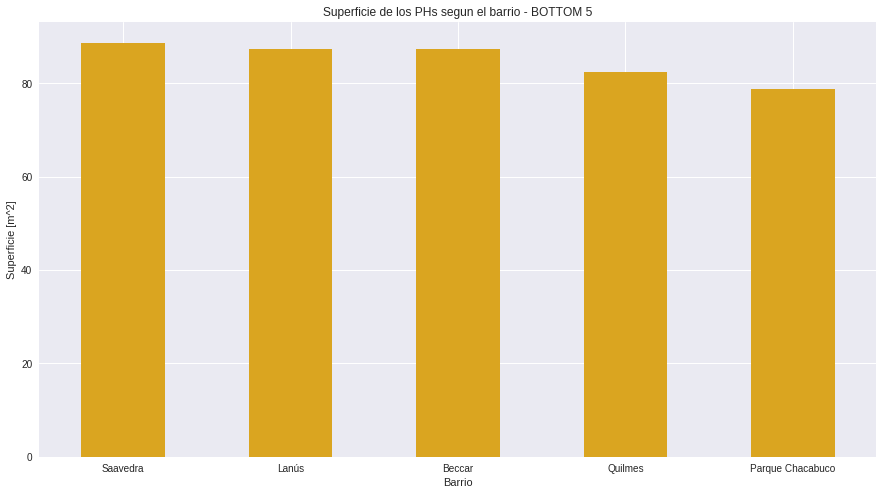
\includegraphics[width=\textwidth]{../images/phSurfaceBottomBar}
				  	\end{center}
				  	\tab En cuanto a la ubicación geográfica, veremos una ubicación de los barrios muy variada:
				  	\begin{center}
   		    				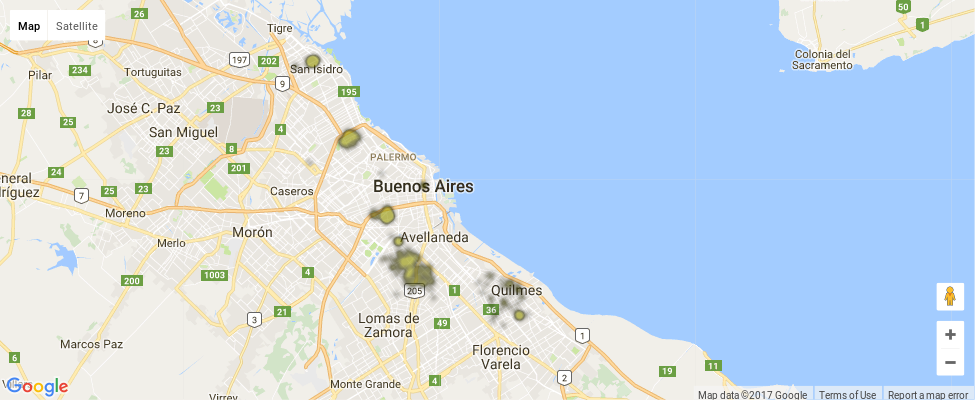
\includegraphics[width=\textwidth]{../images/phSurfaceBottomMap}
				  	\end{center}
				  	\tab Desde Saavedra y Parque Chacabuco en CABA, hasta dos barrios alejados como Beccar en Zona Norte y Quilmes
				  	en Zona Sur.
				\subsubsection{Departamentos}
					El \emph{Bottom 5} de los departamentos está conformado por:
					\begin{center}
						\begin{tabular}{ |c|c|c| }
							\hline
							\multicolumn{3}{|c|}{Superficie promedio de los departamentos por barrio}\\
							\hline
							\hline
							Puesto & Barrio & Superficie [$m^2$]\\
							\hline
							5 & Munro & 50\\
							4 & Villa Luzuriaga & 48\\
							3 & Morón & 48\\
							2 & Parque Chas & 46\\
							1 & Boedo & 40\\
							\hline
						\end{tabular}
					\end{center}
					\tab La superficie promedio para estos departamentos es de aproximadamente la mitad de los PHs más pequeños
					y tienen un promedio menor al $30\%$ de los departamentos más grandes. Aquí encontramos nuevamente a Munro, que
					también se encuentra en el \emph{Bottom 5} de las casas. \\
					\tab Aquí, nuevamente, un gráfico de barras nos dará cinco barras muy similares, con Villa Luzuriaga y Morón
					compartiendo el mismo valor y una diferencia entre el primero y el quinto de sólo  $10m^2$.
					\begin{center}
   		    				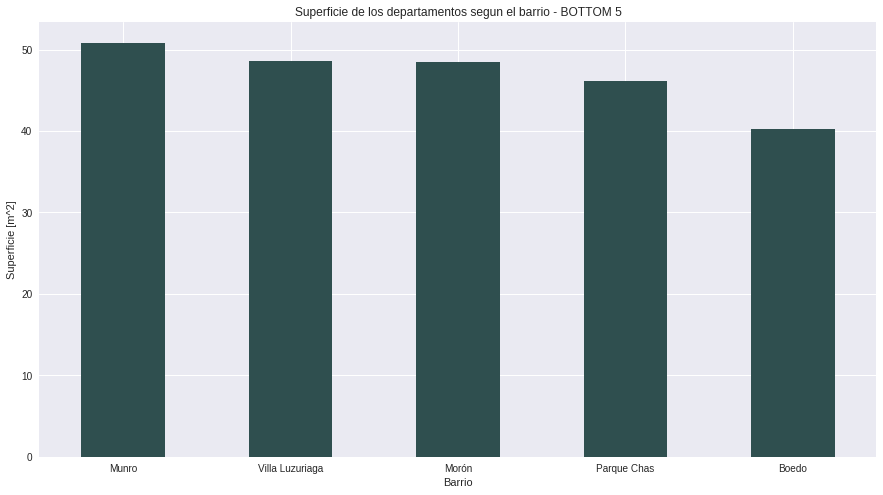
\includegraphics[width=\textwidth]{../images/apartmentSurfaceBottomBar}
				  	\end{center}
				  	\tab En cuanto a la ubicación geográfica, si observamos el siguiente mapa:
				  	\begin{center}
   		    				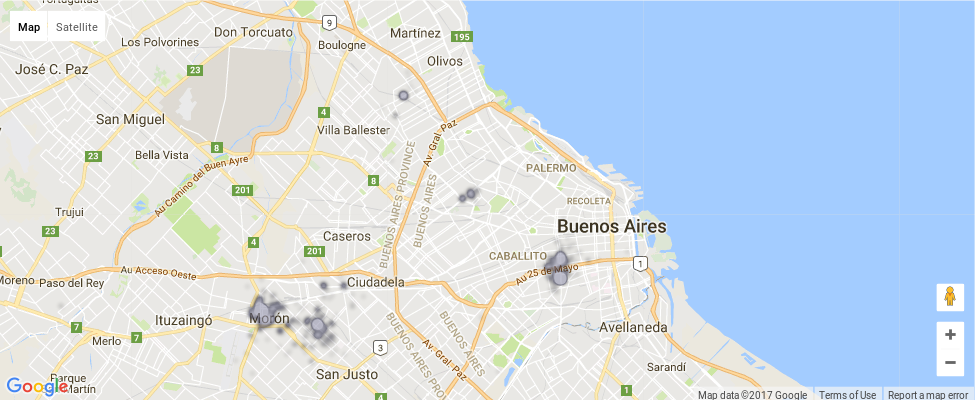
\includegraphics[width=\textwidth]{../images/apartmentSurfaceBottomMap}
				  	\end{center}
				  	\tab Podemos ver que no hay una tendencia particular, pues encontramos barrios dentro de Capital Federal, en la
				  	Zona Norte y en la Zona Oeste, siendo dos los barrios de la última y dos los de la primera.
				\subsubsection{Locales}
					Finalmente, para los locales, el \emph{Bottom 5} es el siguiente:
					\begin{center}
						\begin{tabular}{ |c|c|c| }
							\hline
							\multicolumn{3}{|c|}{Superficie promedio de los locales por barrio}\\
							\hline
							\hline
							Puesto & Barrio & Superficie [$m^2$]\\
							\hline
							5 & Palermo & 145\\
							4 & Ramos Mejía & 125\\
							3 & Villa Crespo & 120\\
							2 & Barrio Norte & 119\\
							1 & Belgrano & 92\\
							\hline
						\end{tabular}
					\end{center}
					\tab Esta tabla nos permite ver que entre los integrantes del \emph{Bottom 5} y los del \emph{Top 5} hay una
					variación del $42\%$, que es la más pequeña entre todos los tipos. \\
					\tab El hecho de que Belgrano sea el más pequeño se lo atribuímos a la cantidad de locales que se pueden
					encontrar en dicho barrio tanto en avenidas como Cabildo o en galerías comerciales en esa misma avenida, en donde
					se encuentran muchísimos locales muy pequeños uno al lado del otro.
					\tab En este caso, el gráfico de barras si mostrará una variación importante, pues Belgrano tiene una
					superficie promedio que representa el $63\%$ de la de Palermo.
					\begin{center}
   		    				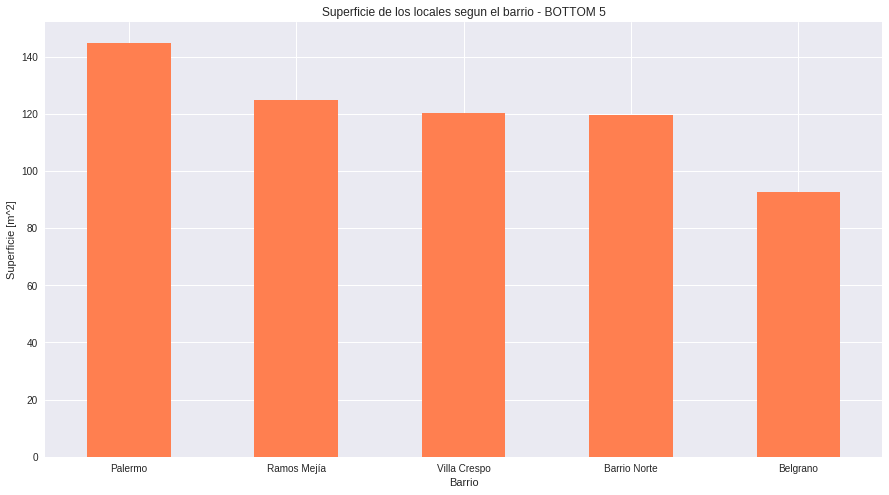
\includegraphics[width=\textwidth]{../images/storeSurfaceBottomBar}
				  	\end{center}
				  	\tab Finalmente, si analizamos la ubicación geográfica de estos barrios, vemos lo siguiente:
				  	\begin{center}
   		    				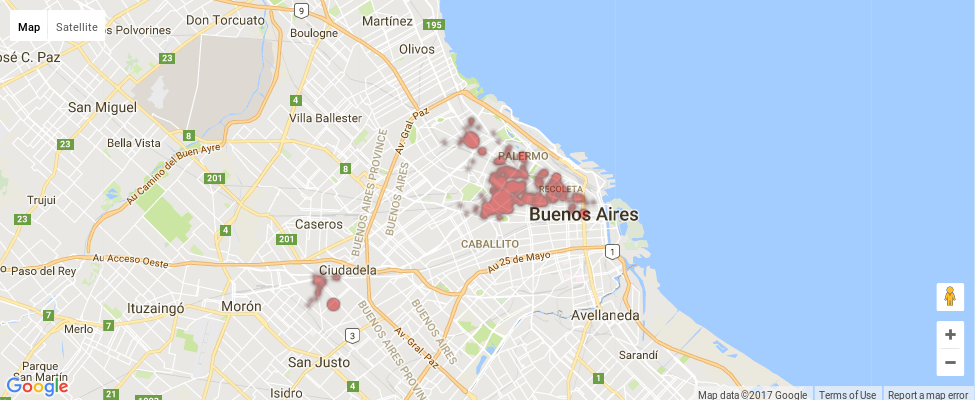
\includegraphics[width=\textwidth]{../images/storeSurfaceBottomMap}
				  	\end{center}
				  	\tab La mayoría de los barrios se encuentran en una zona casi continua del Centro-Norte de Capital Federal con
				  	la excepcion de Ramos Mejía en Zona Oeste. \\
				  	\tab Se puede observar, si se compara con el \emph{Top 5}, se puede ver que los barrios en este último se
				  	encuentran 'de Recoleta para el Sur' y en el caso actual se encuentran 'de Recoleta para el Norte'. 
\end{document}